\documentclass{beamer}
\usepackage{graphicx}
\author{Andrew Johnson}
\date{\today}
\usetheme{Boadilla}
\useinnertheme{rectangles}
\usepackage{hyperref}
\title{This is the title}

\begin{document}

\frame{\titlepage}
\frame{\tableofcontents}

\begin{frame}
\frametitle{This is the frame title}
Frames can consist of plain text, lists (numbered or not), images.
You can have as long of a frame as you want, but no commands
are used to break up long slides.
Math font like $x=y$ is captured natively.
\end{frame}

\begin{frame}
\frametitle{Another frame}
Frames are broken up by empty lines. Contents of a paragraph
can run over multiple lines. If the frame title does not
appear directly above the frame, or at least attached to the block,
the title will not be applied to the desired frame.
\end{frame}

\begin{frame}
\frametitle{Empty frame}
\end{frame}

\begin{frame}
This frame has no title.
Sad frame.
\end{frame}

\section{New section}
\frame{\sectionpage}

\begin{frame}
\frametitle{Lists}
\begin{itemize}
\item{Only single level lists are supported for now}
\item{You can mix symbols and they will be treated as the same bulletted list}
\end{itemize}
\begin{enumerate}
\item{Switching to numbers will terminate the list and switch to enumerations}
\item{Just like markdown, number doesn't matter, just that it's a numeric entry followed by a period and a space}
\item{This is really the third item. The next line is an edge case}
\item{a}
\end{enumerate}
\end{frame}

\begin{frame}
\frametitle{Long lines}
\begin{itemize}
\item{The contents of a single line are passed to a list item}
\item{Line continuation is not supported as each line is treated separately from previous and next lines}
\item{This hopefully discourages very long list items}
\end{itemize}
\end{frame}

\subsection{Subsection}

\begin{frame}
\frametitle{Images too!}
\begin{figure}
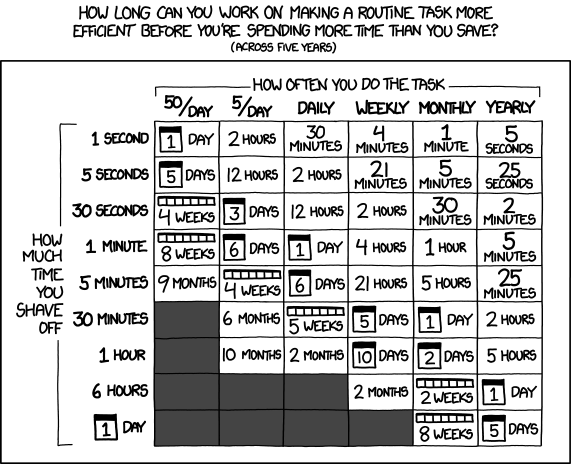
\includegraphics[width=0.6\textwidth,height=0.6\textheight,keepaspectratio]{assets/is_it_worth_the_time.png}
\caption{XKCD 1205 (CC-BY NC 2.5)}
\label{figure0}
Original link: \url{https://xkcd.com/1205/}.
License: \url{https://creativecommons.org/licenses/by-nc/2.5/}
\end{figure}
\end{frame}

\section{Conclusion}

\begin{frame}
\frametitle{Conclusion}
This is a pretty neat tool (I think so).
It has some limits, and there is more to add.
\end{frame}
\end{document}
